%%%%%%%%%%%%%%%%%%%%%%%%%%%%%%%%%%%%%%%%%%%%%%%%%%%%%%%%%%%%%%%%%%%%%%%%%%%%%%%%
% Soutenance de projet - Fichier modèle pour présentations Beamer
%%%%%%%%%%%%%%%%%%%%%%%%%%%%%%%%%%%%%%%%%%%%%%%%%%%%%%%%%%%%%%%%%%%%%%%%%%%%%%%%
\documentclass{beamer}
\usepackage[utf8]{inputenc}
\usepackage[francais]{babel}
\usepackage[T1]{fontenc}
\usepackage{textcomp}
\usepackage{relsize}
\usepackage{amssymb}
\usepackage{framed}
% \usepackage{makeidx}


%%% THÈME TORINO AVEC MINIFRAMES MODIFIÉES - NÉCESSITE FICHIERS SPÉCIAUX
\usetheme[pageofpages=sur,% String used between the current page and the
                         % total page count.
          alternativetitlepage=true,% Use the fancy title page.
          titlepagelogo=logo,% Logo for the first page.
          titleline=true,
          watermark=watermark,% Watermark used in every page.
          watermarkheight=100px,% Height of the watermark.
          watermarkheightmult=4,% The watermark image is 4 times bigger
                                % than watermarkheight.
          ]{Torino}
\useoutertheme[subsection=true]{miniframes2}
\usecolortheme{freewilly}
%%% FIN DU SECOND THÈME

% Add images path to graphics default include path
\graphicspath{{images/}}

% nouvelle commande pour un joli nom
\newcommand{\nom}[1]{\textsc{#1}}

% commande pour une zolie ligne
\newcommand{\ligne}[1][1pt]{
  \par\noindent
  \rule[.5ex]{\linewidth}{#1}\par}

% \0
\newcommand{\slz}{$\backslash0$}

\newcommand{\executeiffilenewer}[3]{%
 \ifnum\pdfstrcmp{\pdffilemoddate{#1}}%
 {\pdffilemoddate{#2}}>0%
 {\immediate\write18{#3}}\fi%
}

\newcommand{\includesvg}[2]{%
 \executeiffilenewer{#1.svg}{#1.pdf}%
 {inkscape -z -D --file=#1.svg --export-pdf=#1.pdf --export-width=1000}%
% \input{#1.eps_tex}%
 \includegraphics[scale=#2]{#1.pdf}
}

\newcommand{\includedot}[2]{%
 \executeiffilenewer{#1.dot}{#1.pdf}%
 {dot -T pdf -o #1.pdf #1.dot}%
 %\input{#1.eps_tex}%
 \includegraphics[scale=#2]{#1.pdf}
}

\newcommand{\includepic}[2]{%
 \immediate\write18{pic2plot -Tsvg --bg-color none #1.pic > #1.svg && inkscape -z -D --file=#1.svg --export-pdf=#1.pdf --export-width=1000}%
 \includegraphics[scale=#2]{#1.pdf}
}

%%% TITRE DE PAGE
\title{Intégration de PIGA dans le noyau Linux}
\subtitle{Projet recherche 2011 -- 2012}
\author{Timothée~Ravier}
\institute{ENSI de Bourges}
\date{16 décembre 2011}

%%% POUR AVOIR UN PLAN QUI S'AFFICHE QUAND ON CHANGE DE SOUS-SECTION
\AtBeginSection[ ]
{
 \begin{frame}<beamer>
   \frametitle{Plan}
   \tableofcontents[currentsection]
  \end{frame}
}
\NoAutoSpaceBeforeFDP

\begin{document}

%%% LA PAGE DE TITRE, ON PEUT Y APPLIQUER DES OPTIONS COMME INSTITUTE CI-DESSOUS
{
	\framenumberoff
	\watermarkoff
	\institute{École Nationale Supérieure d'Ingénieurs de Bourges} % Vire le champ institut sur cette page
	\begin{frame}
	\titlepage
	\end{frame}
}

\section{SELinux et PIGA}
\begin{frame}{SELinux et PIGA}
	Principe d'une protection système avancée
	\begin{itemize}
		\item Propriétés de sécurité évoluées
		\item Base de signatures
		\item Contrôle de ces activités
	\end{itemize}
	\vspace{-1cm}
	\hspace{1cm}
		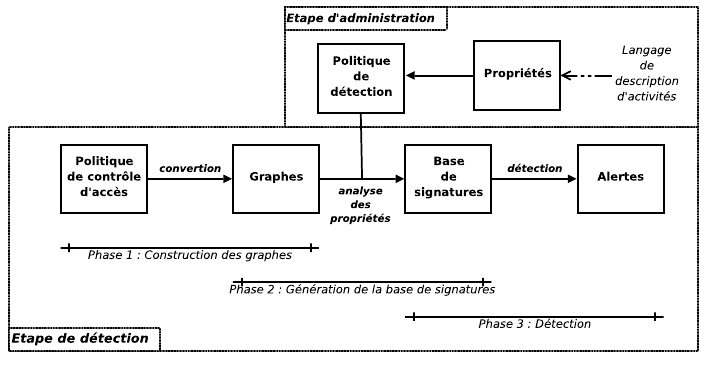
\includegraphics[scale=0.5]{piga_principe.png}
\end{frame}

\section{Intégration dans le noyau}
\begin{frame}{Intégration dans le noyau}
	\begin{center}
		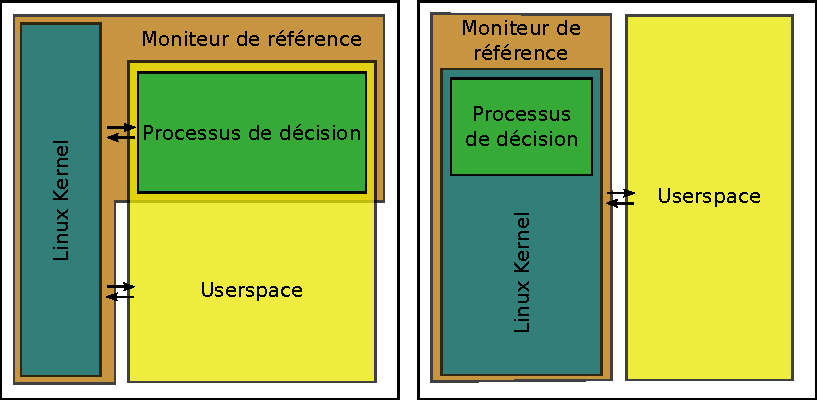
\includegraphics[scale=0.8]{piga_evol.pdf}
	\end{center}
	\vspace{-0.5cm}
	\begin{itemize}
		\item meilleures performances
		\item robustesse (attaques sur le moniteur de référence plus difficile)
	\end{itemize}
\end{frame}

\section{Démonstration}
\begin{frame}
	\frametitle{Démonstration}
\end{frame}

\end{document}
